% Compile with XeLaTeX !!
\documentclass[12pt,a4paper]{article}

% -------------------------------------------------
% Fonts & Greek language via polyglossia
% -------------------------------------------------
\usepackage{fontspec}
\usepackage{polyglossia}

\setmainlanguage{greek}
\setotherlanguage{english}

\setmainfont{Times New Roman}
\setsansfont{Arial}
\setmonofont{Courier New}

% -------------------------------------------------
% Math & Formatting
% -------------------------------------------------
\usepackage{amsmath, amssymb, amsfonts}
\usepackage{geometry}
\usepackage{float}
\usepackage{hyperref}
\usepackage{caption}
\usepackage{graphicx}
\usepackage{multirow}
\usepackage{multirow}

\geometry{margin=2.5cm}

\title{\textbf{Τεχνικές Βελτιστοποίησης}\\
	\large 3η Εργαστηριακή Άσκηση}
\author{Πελοπίδας-Νικόλαος Τσιούντσιουρας \\ ΑΕΜ: 11085}
\date{\today}
\setcounter{tocdepth}{3}

\begin{document}
	
	\maketitle
	\tableofcontents
	\newpage
	
	% ======================================================
	% 1. Εισαγωγή
	% ======================================================
	\section{Εισαγωγή}
	
	Η παρούσα εργαστηριακή άσκηση αφορά την εφαρμογή και μελέτη της μεθόδου Μέγιστης Καθόδου, καθώς και της εκδοχής της με Προβολή, σε μια κυρτή
	τετραγωνική συνάρτηση της μορφής
	\[
	f(x)=\frac{1}{3}x_1^2+3x_2^2.
	\]
	Αρχικά εξετάζουμε την άνευ περιορισμών ελαχιστοποίηση για διάφορες σταθερές τιμές βήματος $\gamma$, ενώ στη συνέχεια προσθέτουμε περιορισμούς και εφαρμόζουμε
	προβολή στο εφικτό σύνολο.
	
	Στόχος είναι η παρατήρηση της επίδρασης της επιλογής βήματος και των παραμέτρων του αλγορίθμου στη σύγκλιση. Τα αποτελέσματα παρουσιάζονται συγκριτικά μέσω πειραμάτων	και σχολιάζονται συνοπτικά στο τέλος της αναφοράς.

	% ======================================================
	% 2. Θεωρία
	% ======================================================
	\section{Θεωρία}
	
	Στην ενότητα αυτή παρουσιάζονται συνοπτικά οι βασικές αρχές των αλγορίθμων που χρησιμοποιήθηκαν στην εργασία. Αρχικά εξετάζεται η μέθοδος Μέγιστης Καθόδου για προβλήματα χωρίς περιορισμούς, και στη συνέχεια η αντίστοιχη μέθοδος με Προβολή σε εφικτό σύνολο.
	
	\subsection{Μέθοδος Μέγιστης Καθόδου}
	Σε κάθε επανάληψη της μεθόδου \textbf{Μέγιστης Καθόδου} ο	αλγόριθμος κινείται προς την αρνητική κατεύθυνση της κλίσης της αντικειμενικής συνάρτησης, επιλέγοντας τοπικά την κατεύθυνση με τον μεγαλύτερο ρυθμό μείωσης. Η απόδοση της μεθόδου εξαρτάται σε μεγάλο βαθμό από την επιλογή του μήκους βήματος.
	
	Αναλυτικά ο αλγόριθμος:
	\paragraph{Αρχικοποίηση} Ορίστε $\epsilon>0$ τη σταθερά τερματισμού. Επιλέξτε το αρχικό σημείο $x_1$ και θέστε $k=1$.
	\paragraph{Κύριο Βήμα} Αν $|\nabla f(x_k)|<\epsilon$ ο αλγόριθμος τερματίζει. Διαφορετικά, θέστε $d_k=-\nabla f(x_k)$. Θέστε $x_{k+1}=x_k-\gamma_k\nabla f(x_k)$, $k=k+1$, όπου $\gamma$ δοσμένη σταθερά, και επαναλάβετε το κυρίως βήμα.
	
	\subsection{Μέθοδος Μέγιστης Καθόδου με Προβολή}
	
	Η μέθοδος Μέγιστης Καθόδου με Προβολή επεκτείνει την κλασική μέθοδο σε προβλήματα με περιορισμούς, προβάλλοντας σε κάθε βήμα το νέο σημείο στο εφικτό σύνολο. Με αυτόν τον τρόπο διασφαλίζεται ότι οι επαναλήψεις παραμένουν εντός των επιτρεπτών ορίων, ενώ η διαδικασία αναζήτησης ακολουθεί και πάλι την κατεύθυνση της μέγιστης καθόδου ανά επανάληψη.
	
	Αναλυτικά ο αλγόριθμος:
	\paragraph{Βήμα 1} Ξεκινήστε με ένα εφικτό σημείο $x_0 \in X$
	\paragraph{Βήμα 2} Ακολουθήστε τη μέθοδο Μέγιστης Καθόδου για την ελαχιστοποίηση της $f$.
	\paragraph{Βήμα 3} Αν το νέο σημείο είναι εφικτό, συνεχίστε με την ίδια μέθοδο.
	\paragraph{Βήμα 4} Αν το νέο σημείο δεν είναι εφικτό, βρείτε την προβολή του στο $X$ και πηγαίνετε στο Βήμα 2 μέχρι να καταλήξετε σε στάσιμο σημείο.
	
	% ======================================================
	% 3. Πειράματα
	% ======================================================
	\section{Πειράματα}
	
	\subsection{Μέθοδος Μέγιστης Καθόδου για Διαφορετικά $\gamma$}
	\subsubsection{Αναλυτική εξέλιξη επαναλήψεων}
	Για τη συνάρτηση
	\[
	f(x_1,x_2)=\frac{1}{3}x_1^2+3x_2^2
	\]
	η κλίση είναι
	\[
	\nabla f(x)=\begin{pmatrix}
		\frac{2}{3}x_1\\
		6x_2
	\end{pmatrix},
	\]
	οπότε ο αλγόριθμος Μέγιστης Καθόδου με σταθερό βήμα $\gamma$ γράφεται
	\[
	x_{k+1}=x_k-\gamma \nabla f(x_k),
	\]
	δηλαδή
	\[
	x_{1}^{k+1}=\Bigl(1-\frac{2\gamma}{3}\Bigr)x_{1}^{k},\qquad
	x_{2}^{k+1}=(1-6\gamma)x_{2}^{k},
	\]
	άρα
	\[
	x_1^k=\Bigl(1-\frac{2\gamma}{3}\Bigr)^k x_1^0,\qquad
	x_2^k=(1-6\gamma)^k x_2^0.
	\]
	
	Η σύγκλιση στο ελάχιστο σημείο $(0,0)$ απαιτεί
	\[
	\Bigl|1-\frac{2\gamma}{3}\Bigr|<1
	\quad\text{και}\quad
	|1-6\gamma|<1,
	\]
	οπότε τελικά
	\[
	0<\gamma<\frac{1}{3}.
	\]
	Επομένως για $\gamma=0.1$ και $\gamma=0.3$ η μέθοδος συγκλίνει, ενώ για
	$\gamma=3$ και $\gamma=5$ αναμένεται απόκλιση, κάτι που επιβεβαιώνεται και
	από τα πειραματικά αποτελέσματα.
	
	% ------------------------------------------------------------------
	\paragraph{Περίπτωση $\gamma=0.1$}
	Στην περίπτωση του πολύ μικρού βήματος η μέθοδος συγκλίνει μεν, ωστόσο το
	ποσοστό μείωσης της $f(x_k)$ είναι σχετικά αργό και απαιτούνται αρκετές
	επαναλήψεις μέχρι την επίτευξη του κριτηρίου τερματισμού. Η σύγκλιση είναι
	σταθερή και χωρίς ταλαντώσεις.
	
	\begin{figure}[H]
		\centering
		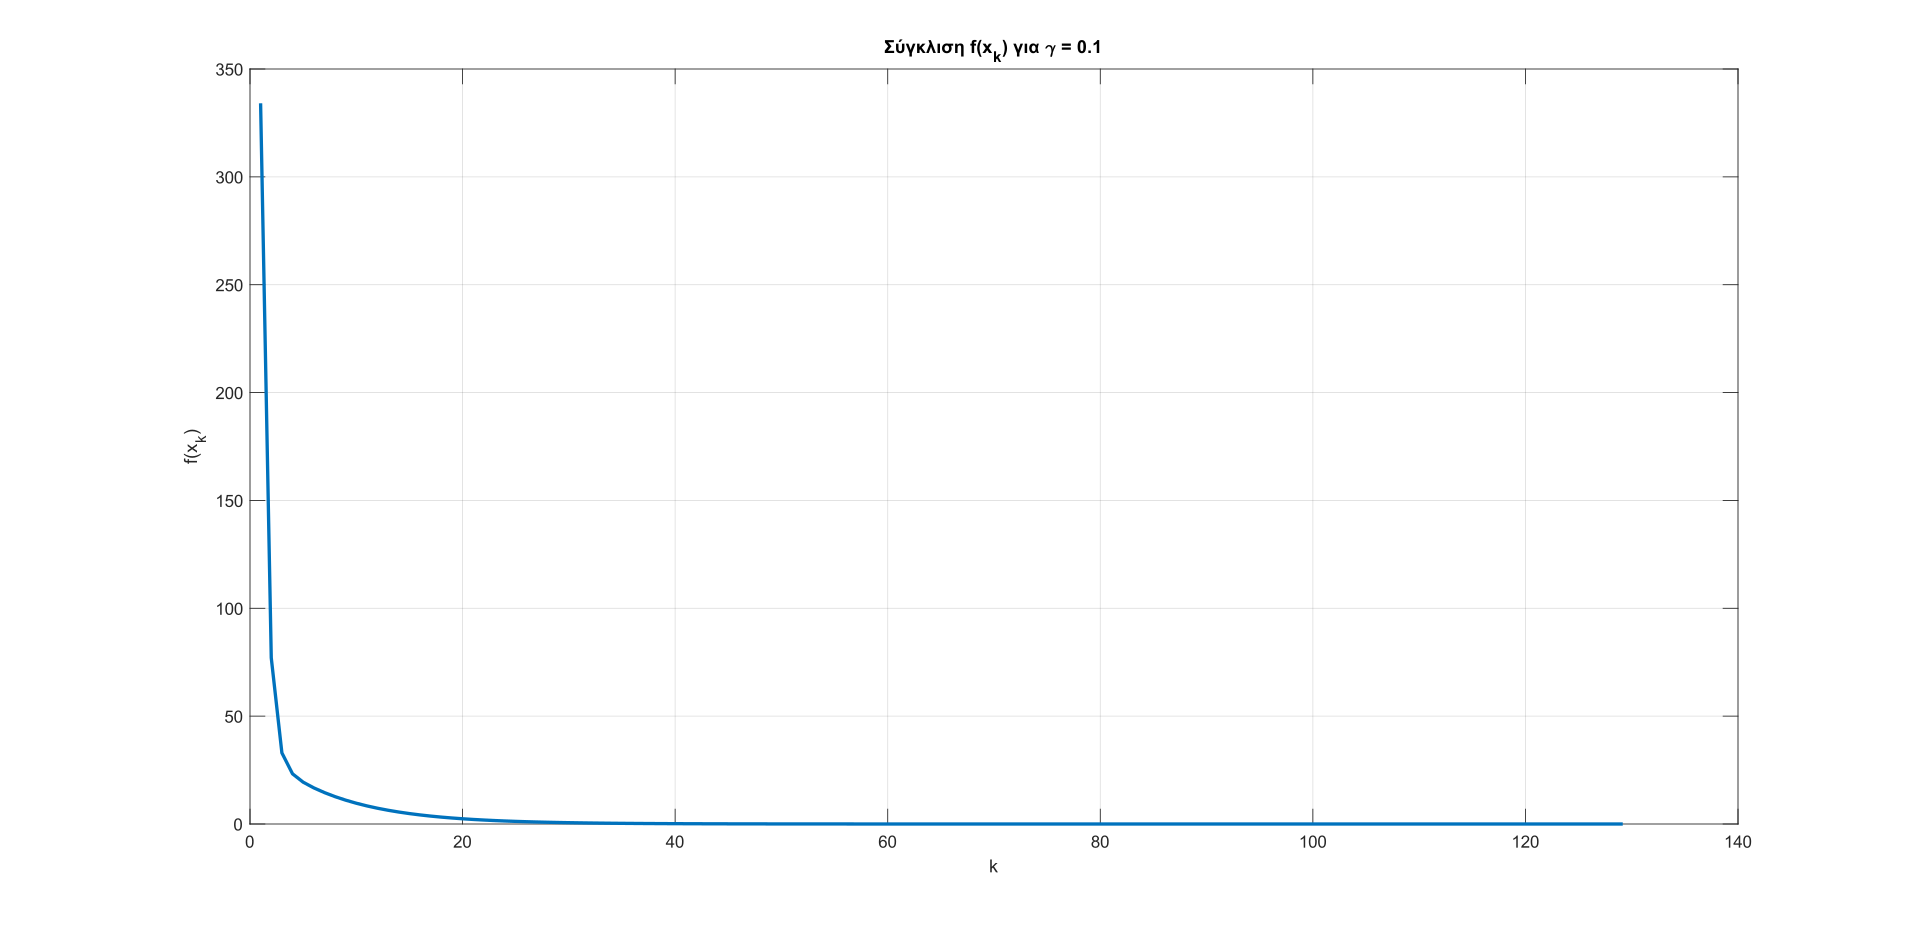
\includegraphics[width=0.8\textwidth]{exercise_1/convergence_f_01.png}
		\caption{Σύγκλιση της $f(x_k)$ για $\gamma=0.1$.}
	\end{figure}
	
	\begin{figure}[H]
		\centering
		\includegraphics[width=0.8\textwidth]{exercise_1/convergence_plot_01.png}
		\caption{Τροχιά σύγκλισης για $\gamma=0.1$.}
	\end{figure}
	
	
	% ------------------------------------------------------------------
	\paragraph{Περίπτωση $\gamma=0.3$}
	Για $\gamma=0.3$ παρατηρείται ταχύτερη μείωση της $f(x_k)$ και σημαντικά
	λιγότερες απαιτούμενες επαναλήψεις. Παράλληλα όμως, εμφανίζονται μικρές
	ταλαντώσεις κοντά στο σημείο ελαχίστου, καθώς το βήμα είναι μεγαλύτερο και πιο
	κοντά στο όριο σταθερότητας.
	
	\begin{figure}[H]
		\centering
		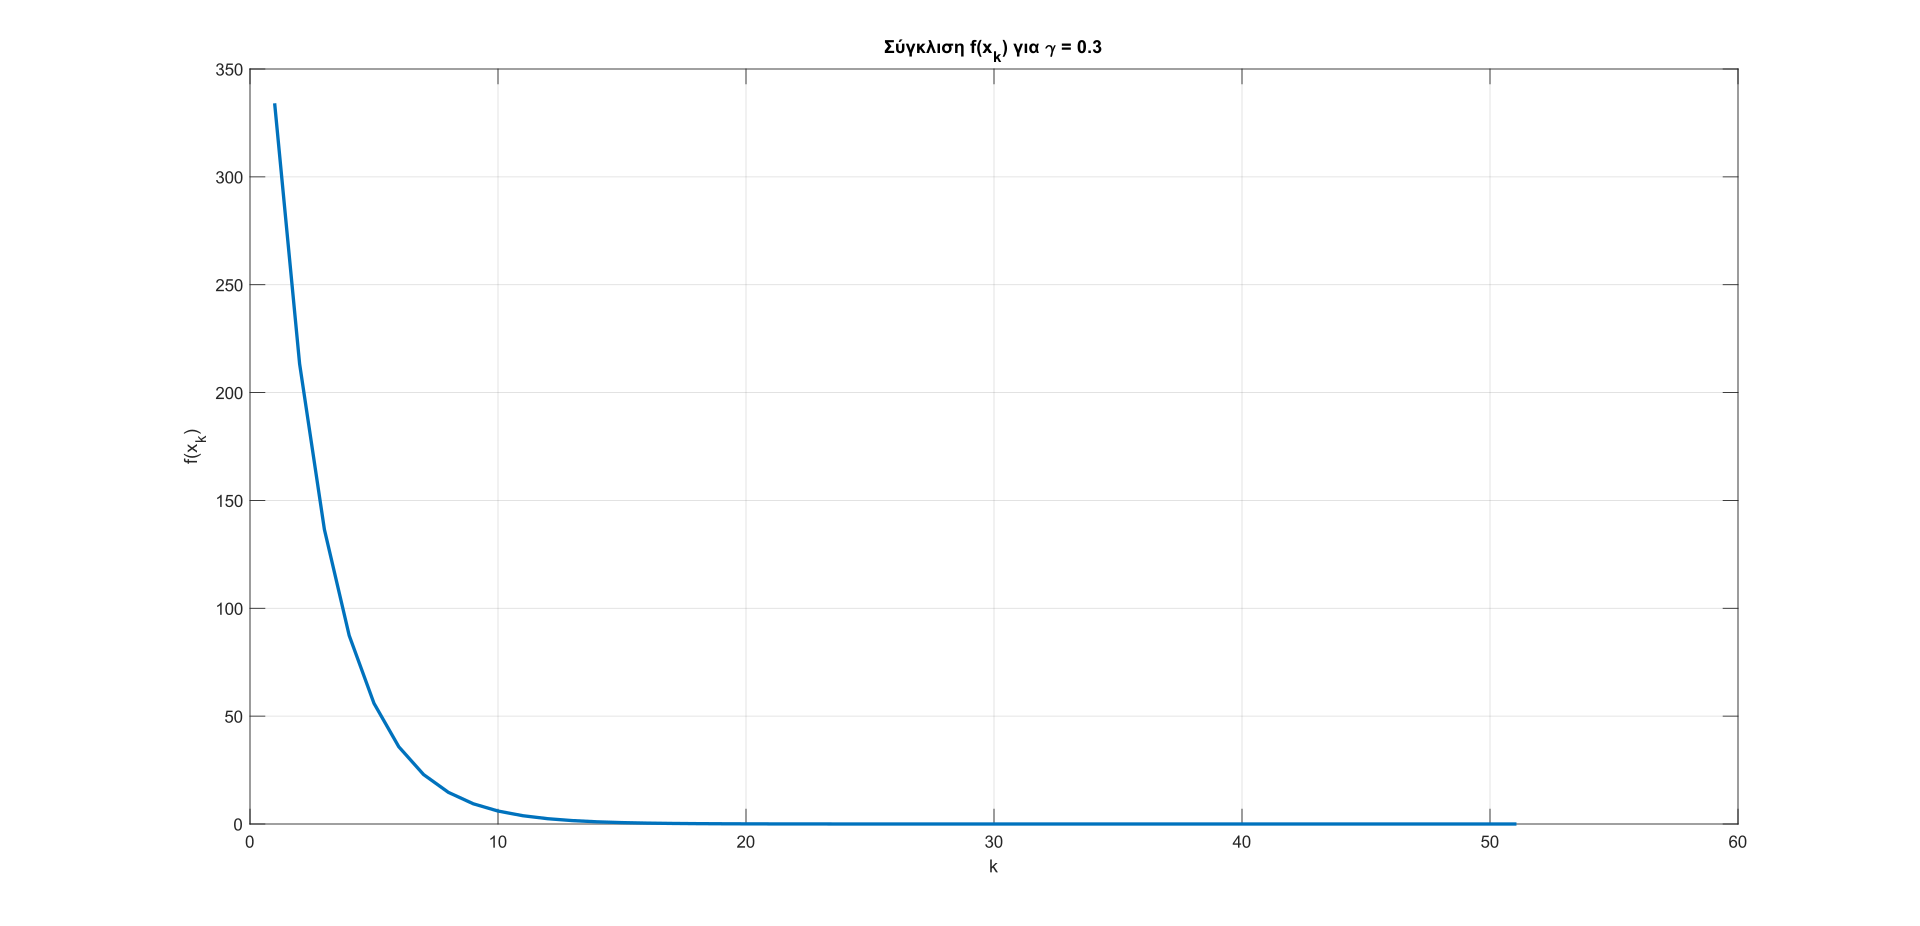
\includegraphics[width=0.8\textwidth]{exercise_1/convergence_f_03.png}
		\caption{Σύγκλιση της $f(x_k)$ για $\gamma=0.3$.}
	\end{figure}
	
	\begin{figure}[H]
		\centering
		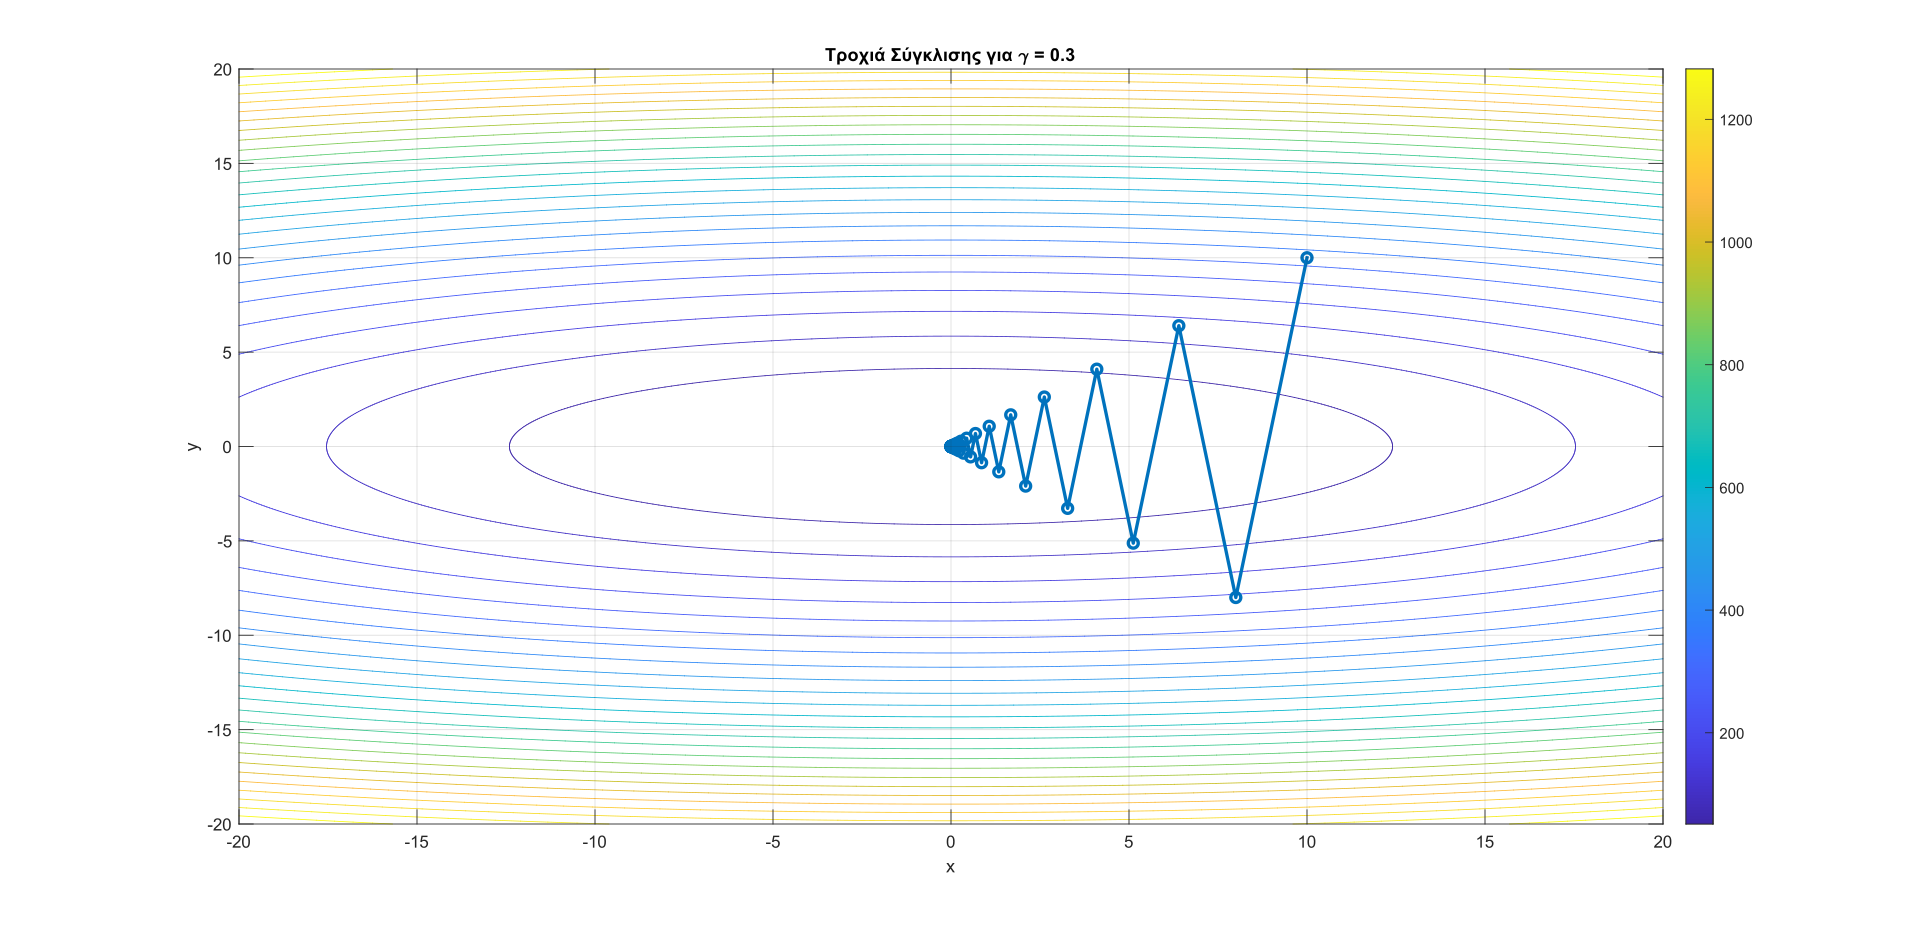
\includegraphics[width=0.8\textwidth]{exercise_1/convergence_plot_03.png}
		\caption{Τροχιά σύγκλισης για $\gamma=0.3$.}
	\end{figure}
	
	
	% ------------------------------------------------------------------
	\paragraph{Περίπτωση $\gamma=3$}
	Για $\gamma=3$ η μέθοδος δεν συγκλίνει. Η τιμή της $f(x_k)$ αυξάνεται
	ραγδαία μετά από ελάχιστες επαναλήψεις, φαινόμενο που υποδηλώνει πλήρη
	αστάθεια της μεθόδου για αυτή την τιμή βήματος.
	
	\begin{figure}[H]
		\centering
		\includegraphics[width=0.8\textwidth]{exercise_1/convergence_f_3.png}
		\caption{Πορεία της $f(x_k)$ για $\gamma=3$.}
	\end{figure}
	
	\begin{figure}[H]
		\centering
		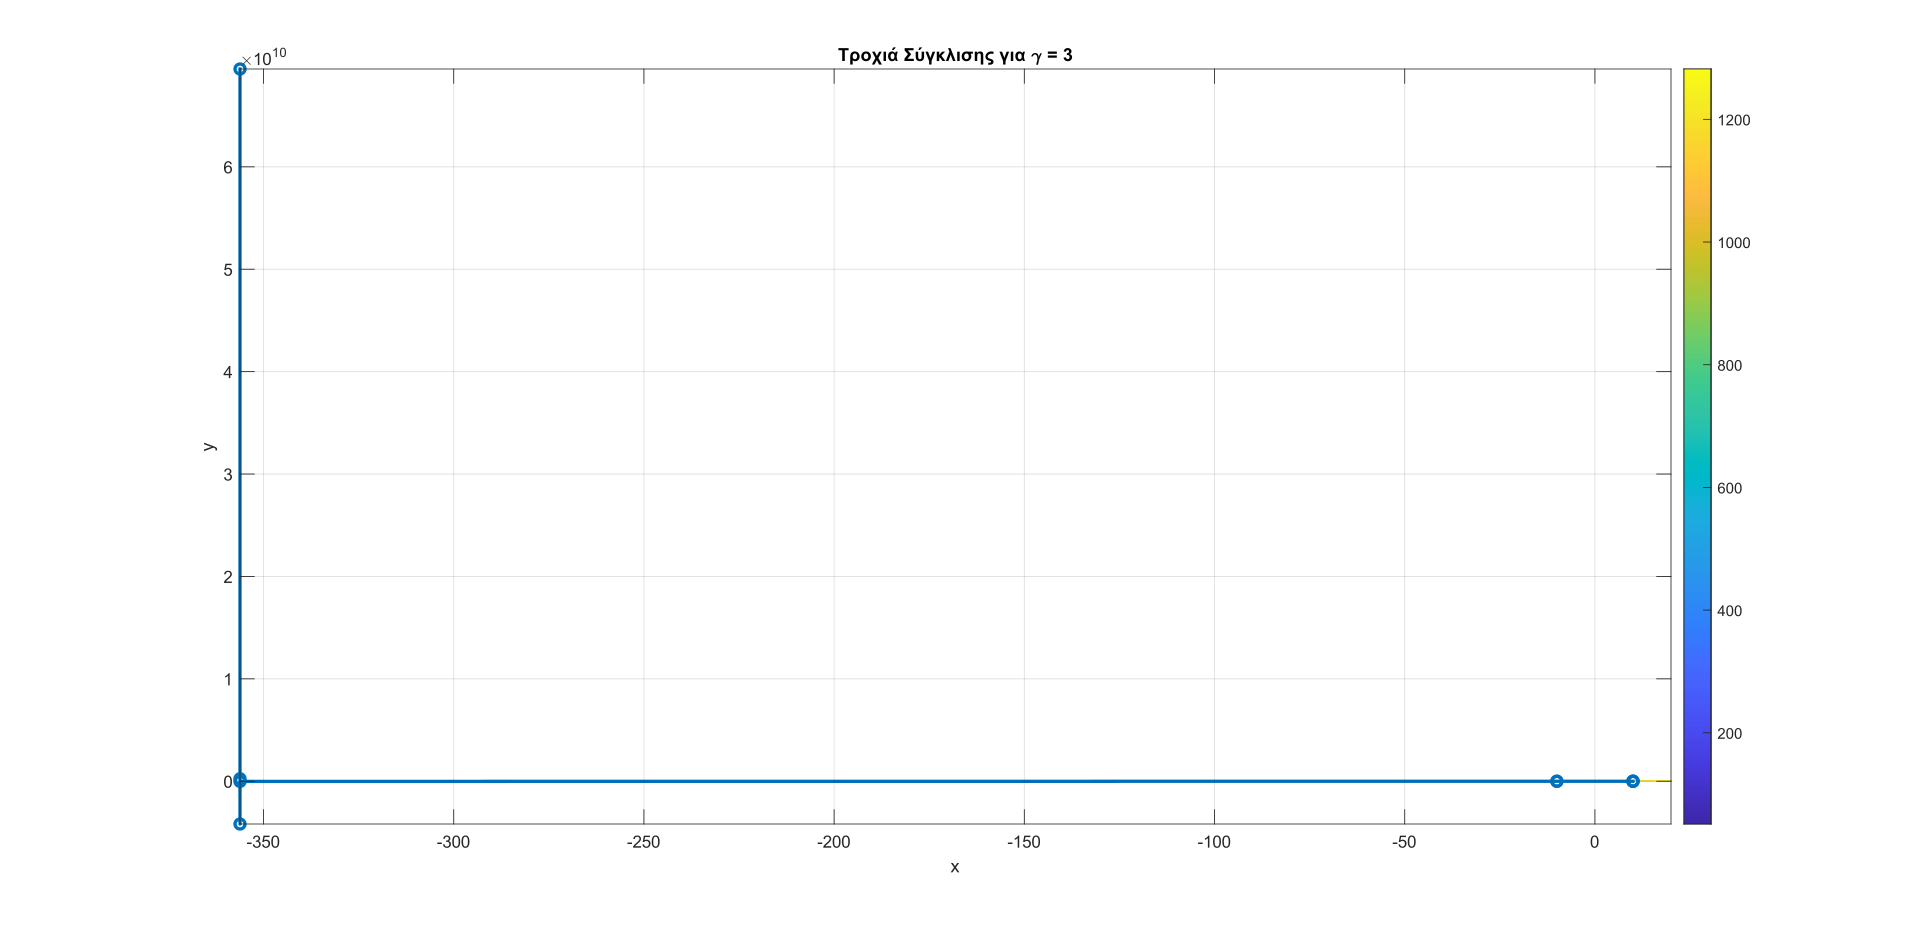
\includegraphics[width=0.8\textwidth]{exercise_1/convergence_plot_3.png}
		\caption{Τροχιά των $x_k$ για $\gamma=3$.}
	\end{figure}
	
	
	% ------------------------------------------------------------------
	\paragraph{Περίπτωση $\gamma=5$}
	Αντίστοιχη συμπεριφορά παρατηρείται και για $\gamma=5$, όπου η μέθοδος
	αποκλίνει ακόμη ταχύτερα. Η τιμή της $f(x_k)$ εκτοξεύεται από τα πρώτα
	βήματα, χωρίς ουσιαστική προσέγγιση του ελάχιστου.
	
	\begin{figure}[H]
		\centering
		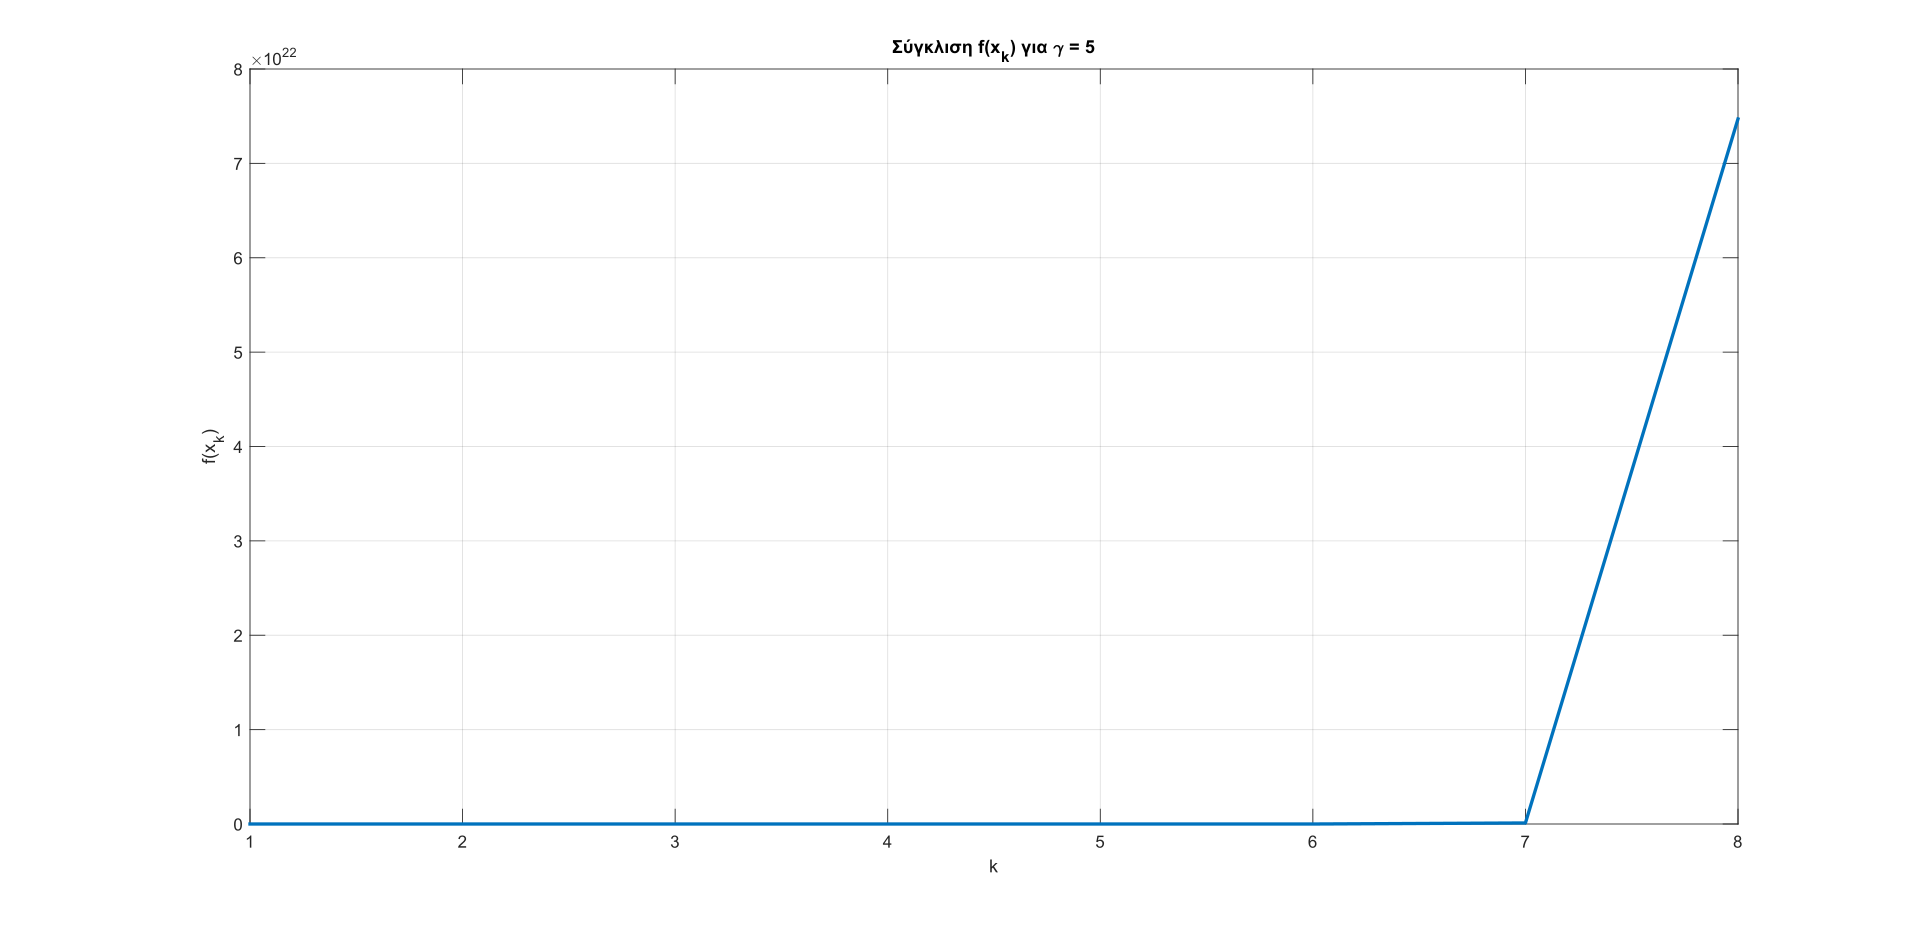
\includegraphics[width=0.8\textwidth]{exercise_1/convergence_f_5.png}
		\caption{Πορεία της $f(x_k)$ για $\gamma=5$.}
	\end{figure}
	
	\begin{figure}[H]
		\centering
		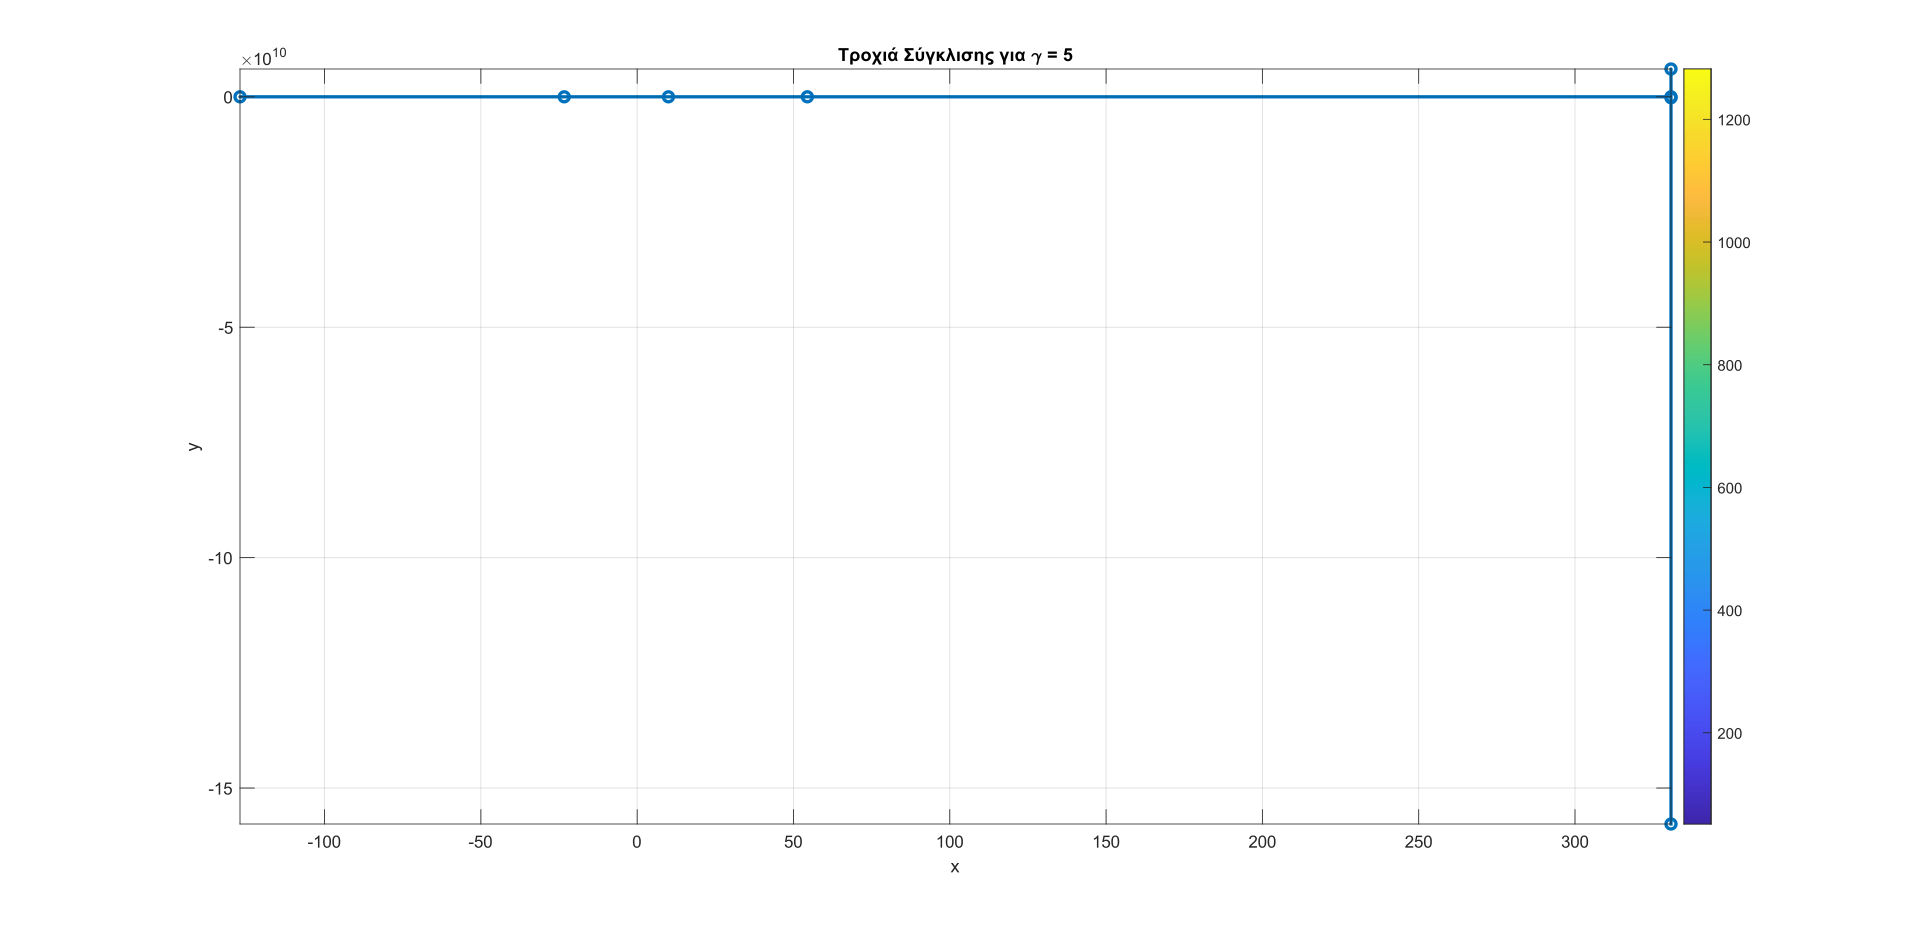
\includegraphics[width=0.8\textwidth]{exercise_1/convergence_plot_5.png}
		\caption{Τροχιά των $x_k$ για $\gamma=5$.}
	\end{figure}
	
	
	% ------------------------------------------------------------------
	\subsubsection{Συγκριτική παρατήρηση}
	Συγκεντρωτικά, η τιμή $\gamma=0.3$ παρουσιάζει τη γρηγορότερη σύγκλιση από τις
	τιμές που οδήγησαν σε σταθερή συμπεριφορά, ενώ η περίπτωση $\gamma=0.1$ είναι η
	πλέον ασφαλής αλλά ιδιαίτερα αργή. Για τις τιμές $\gamma\geq 3$ η μέθοδος
	αποκλίνει πλήρως, γεγονός το οποίο επιβεβαιώνεται και θεωρητικά από το κριτήριο
	σταθερότητας της μεθόδου.
	
	\begin{figure}[H]
		\centering
		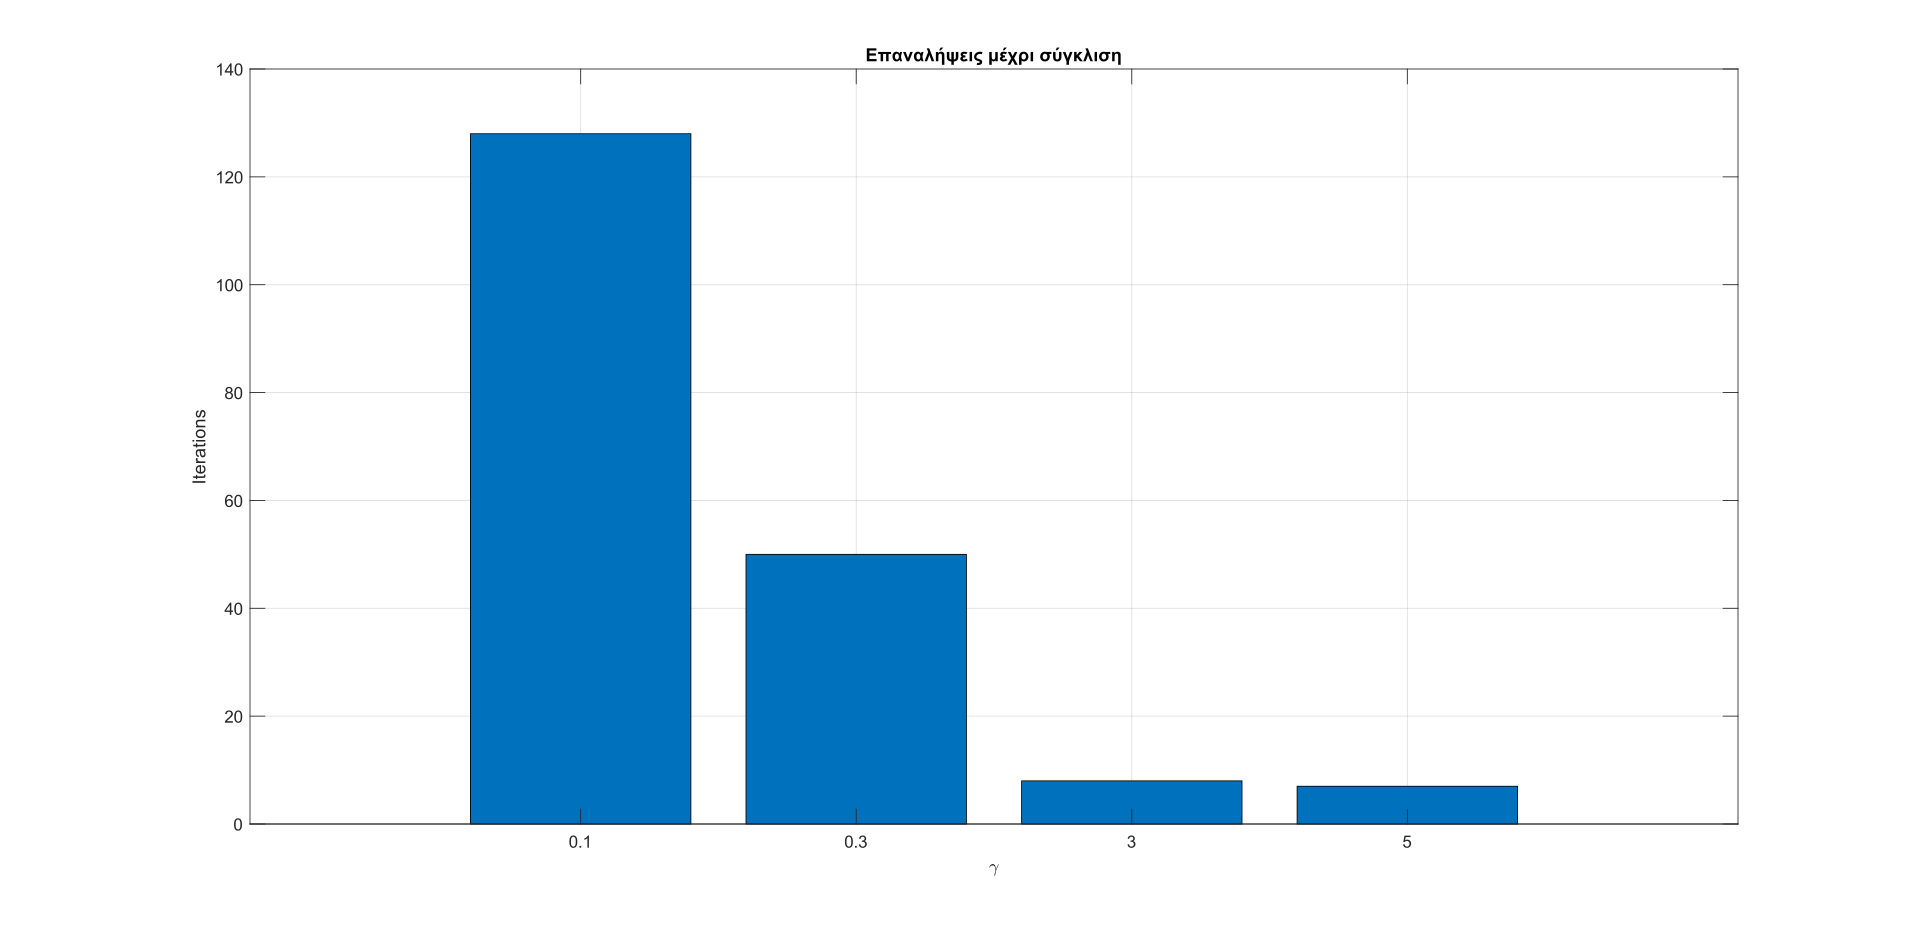
\includegraphics[width=0.8\textwidth]{exercise_1/iterations.png}
		\caption{Επαναλήψεις μέχρι σύγκλιση για διαφορετικές τιμές $\gamma$.}
	\end{figure}
	
	
	\subsection{Μέθοδος Μέγιστης Καθόδου με Προβολή}
	
	Στην περίπτωση όπου το πρόβλημα συνοδεύεται από περιορισμούς,
	η κλασική μέθοδος μέγιστης καθόδου ενδέχεται να παράγει σημεία εκτός του
	εφικτού συνόλου. Η εκδοχή με προβολή αντιμετωπίζει αυτό το ζήτημα
	προβάλλοντας σε κάθε επανάληψη το $x_{k+1}$ στο σύνολο των επιτρεπτών λύσεων,
	εξασφαλίζοντας ότι όλες οι επαναλήψεις παραμένουν εφικτές και η διαδικασία
	οδηγείται προς ένα επιτρεπτό ελάχιστο.
	
	\subsubsection{Περίπτωση $x_0=(5,-5)$, $s_k=5$, $\gamma=0.5$}
	
	Στο δεύτερο πείραμα εξετάζουμε την εφαρμογή της Μεθόδου Μέγιστης Καθόδου με
	Προβολή στο σύνολο των εφικτών λύσεων, με σταθερό βήμα $\gamma=0.5$, σταθερό
	διάνυσμα $s_k=5$ και αρχικό σημείο $x_0=(5,-5)$, έως ότου $\|x_{k+1}-x_k\|
	\leq \varepsilon=10^{-2}$. Η προβολή έχει ως στόχο να εξασφαλίζει ότι κάθε
	νέο σημείο παραμένει εντός του εφικτού συνόλου, ακόμη και στην περίπτωση που η
	κατεύθυνση της βαθμίδας οδηγεί αρχικά εκτός αυτού.
	
	\paragraph{Συμπεριφορά της $f(x_k)$}
	Στο σχήμα που ακολουθεί φαίνεται ότι η τιμή της $f(x_k)$ δεν μειώνεται
	μονοτονικά, αλλά παρουσιάζει έντονες ταλαντώσεις σε ένα εύρος τιμών. Σε
	αντίθεση με το αντίστοιχο πείραμα του Θέματος~1, όπου για κατάλληλες τιμές
	του $\gamma$ παρατηρήθηκε καθοδική πορεία της συνάρτησης, εδώ η μέθοδος δεν
	οδηγεί σε σύγκλιση προς το ελάχιστο.
	
	\begin{figure}[H]
		\centering
		\includegraphics[width=0.8\textwidth]{exercise_2/convergence_f.png}
		\caption{Σύγκλιση της $f(x_k)$ για $\gamma=0.5$ και $s_k=5$.}
	\end{figure}
	
	\paragraph{Τροχιά των επαναλήψεων}
	Ανάλογη συμπεριφορά εμφανίζεται και στην τροχιά των σημείων $(x_k)$,
	όπου παρατηρείται ταλάντωση γύρω από μία περιοχή του εφικτού συνόλου,
	χωρίς σαφή πορεία προς το σημείο ελαχίστου. Η προβολή συγκρατεί τα σημεία
	εντός των περιορισμών, χωρίς όμως να αρκεί για τη σταθεροποίηση της μεθόδου.
	
	\begin{figure}[H]
		\centering
		\includegraphics[width=0.8\textwidth]{exercise_2/convergence_plot.png}
		\caption{Τροχιά σύγκλισης για $\gamma=0.5$ και $s_k=5$.}
	\end{figure}
	
	\paragraph{Συγκριτικό σχόλιο με το Θέμα~1}
	Σε αντίθεση με την μη φραγμένη περίπτωση, η ύπαρξη περιορισμών και η
	προβολή προκαλούν έντονες αναπηδήσεις πάνω στο σύνορο, οι οποίες οδηγούν σε
	ταλαντώσεις της μεθόδου. Συνεπώς, η επιλογή μεγάλου βήματος $\gamma$
	παραμένει κρίσιμη ακόμη και στην προβολική εκδοχή της μεθόδου, καθώς μπορεί
	να αποτρέψει την επίτευξη σύγκλισης, παρότι όλα τα σημεία παραμένουν
	εφικτά. Η παρατήρηση αυτή συμφωνεί με την θεωρία, σύμφωνα με την οποία η
	προβολή δεν εγγυάται σύγκλιση αν το βήμα δεν είναι κατάλληλο.
	
	\subsubsection{Περίπτωση $x_0=(-5,10)$, $s_k=15$, $\gamma_k=0.1$}
	
	Στην περίπτωση αυτή χρησιμοποιούμε τη μέθοδο Μέγιστης Καθόδου με Προβολή με
	σταθερό βήμα $\gamma_k=0.1$, σταθερό $s_k=15$ και αρχικό σημείο
	$x_0=(-5,10)$, μέχρι ακρίβεια $\varepsilon=10^{-2}$.
	
	\paragraph{Συμπεριφορά της $f(x_k)$}
	Όπως φαίνεται στο αντίστοιχο διάγραμμα, η $f(x_k)$ μειώνεται πολύ γρήγορα
	κατά τις πρώτες επαναλήψεις, από μεγάλες τιμές σε τιμές κοντά στο μηδέν.
	Στη συνέχεια παρατηρούνται μικρές ταλαντώσεις γύρω από μια πολύ μικρή τιμή,
	χωρίς εκτροπή όπως στην περίπτωση $\gamma=0.5$ του Θέματος~2.
	
	\begin{figure}[H]
		\centering
		\includegraphics[width=0.8\textwidth]{exercise_3/convergence_f.png}
		\caption{Σύγκλιση της $f(x_k)$ για $\gamma_k=0.1$ και $s_k=15$.}
	\end{figure}
	
	\paragraph{Τροχιά των επαναλήψεων}
	Η τροχιά των σημείων $(x_k)$ δείχνει ότι η μέθοδος κινείται σχεδόν ευθύγραμμα
	από το αρχικό σημείο προς την περιοχή του ελαχίστου και στη συνέχεια κάνει
	πολύ μικρές διορθώσεις γύρω από αυτό. Η συμπεριφορά αυτή μοιάζει με εκείνη
	της κλασικής μεθόδου Μέγιστης Καθόδου στο Θέμα~1 για «συντηρητικό» βήμα, σε
	αντίθεση με την έντονη ταλάντωση που είδαμε στο Θέμα~2 για $\gamma=0.5$.
	
	\begin{figure}[H]
		\centering
		\includegraphics[width=0.8\textwidth]{exercise_3/convergence_plot.png}
		\caption{Τροχιά σύγκλισης για $\gamma_k=0.1$ και $s_k=15$.}
	\end{figure}
	
	\paragraph{Σύγκριση με τα Θέματα 1 και 2}
	Σε σχέση με το Θέμα~1, παρατηρούμε παρόμοια σταθερή συμπεριφορά με γρήγορη
	αρχική μείωση της $f$ και χωρίς απόκλιση, γεγονός που οφείλεται στη σχετικά
	μικρή τιμή του βήματος. Σε σχέση με το Θέμα~2, όπου για $\gamma=0.5$ η μέθοδος
	με προβολή παρέμεινε σε κατάσταση έντονης ταλάντωσης, εδώ η επιλογή
	$\gamma_k=0.1$ οδηγεί σε πρακτική σύγκλιση κοντά στο ελάχιστο.
	
	Ένας απλός πρακτικός τρόπος ώστε η μέθοδος να συγκλίνει στο ελάχιστο είναι η
	προσαρμοστική μείωση του βήματος: όταν σε κάποια επανάληψη δεν ισχύει
	$f(x_{k+1}) \leq f(x_k)$, μειώνουμε το βήμα, π.χ.\ θέτοντας
	$\gamma_{k+1} = \gamma_k/2$, και επαναλαμβάνουμε την επανάληψη. Με αυτόν τον
	τρόπο αποφεύγονται οι μεγάλες ταλαντώσεις και η μέθοδος σταθεροποιείται κοντά
	στο ελάχιστο.
	
	\subsubsection{Περίπτωση $x_0=(8,-10)$, $s_k=0.1$, $\gamma_k=0.2$}
	
	Στην περίπτωση αυτή εφαρμόζεται η μέθοδος Μέγιστης Καθόδου με Προβολή με
	σταθερό βήμα $\gamma_k=0.2$, παράγοντα $s_k=0.1$ και αρχικό σημείο
	$x_0=(8,-10)$, μέχρι ακρίβεια $\varepsilon=10^{-2}$. Το εφικτό σύνολο είναι
	ένα κυρτό ``κουτί'', το οποίο περιέχει στο εσωτερικό του το μηδενικό σημείο
	$(0,0)$.
	
	\paragraph{Εκ των προτέρων πληροφορία σύγκλισης}
	Η συνάρτηση
	\[
	f(x_1,x_2)=\frac{1}{3}x_1^2+3x_2^2
	\]
	είναι κυρτή με γραμμικά Lipschitz κλίση και Hessian με μέγιστη ιδιοτιμή
	$\lambda_{\max}=6$. Από τη θεωρία της μεθόδου Προβολικής Μέγιστης Καθόδου
	προκύπτει ότι για σταθερό βήμα $0<\gamma_k<\frac{2}{\lambda_{\max}}=\frac{1}{3}$
	και κλειστό, κυρτό εφικτό σύνολο, ο αλγόριθμος συγκλίνει στο μοναδικό ελάχιστο
	του προβλήματος. Εφόσον $\gamma_k=0.2<\frac{1}{3}$ και το $(0,0)$ είναι
	εσωτερικό σημείο του συνόλου, αναμένουμε εκ των προτέρων σύγκλιση του
	αλγορίθμου προς το $(0,0)$.
	
	\paragraph{Συμπεριφορά της $f(x_k)$}
	Το διάγραμμα της $f(x_k)$ δείχνει ομαλή και σχεδόν μονοτονική μείωση, από
	μεγάλες αρχικές τιμές προς τιμές πολύ κοντά στο μηδέν, χωρίς εμφανείς
	ταλαντώσεις ή εκτροπή. Η σύγκλιση είναι σταθερή, αν και σχετικά αργή λόγω του
	μικρού αποτελεσματικού βήματος $\gamma_k s_k$.
	
	\begin{figure}[H]
		\centering
		\includegraphics[width=0.8\textwidth]{exercise_4/convergence_f.png}
		\caption{Σύγκλιση της $f(x_k)$ για $\gamma_k=0.2$ και $s_k=0.1$.}
	\end{figure}
	
	\paragraph{Τροχιά των επαναλήψεων}
	Στην τροχιά των $(x_k)$ παρατηρείται αρχικά μία κίνηση κατά μήκος του
	συνόρου του εφικτού συνόλου, καθώς το αρχικό σημείο βρίσκεται εκτός αυτού και
	προβάλλεται στην πλησιέστερη εφικτή θέση. Στη συνέχεια η πορεία λυγίζει προς
	το εσωτερικό και κατευθύνεται σταδιακά προς το $(0,0)$. Κοντά στο ελάχιστο οι
	προβολές ουσιαστικά δεν ενεργοποιούνται και ο αλγόριθμος συμπεριφέρεται όπως
	η κλασική μέθοδος Μέγιστης Καθόδου χωρίς περιορισμούς.
	
	\begin{figure}[H]
		\centering
		\includegraphics[width=0.8\textwidth]{exercise_4/convergence_plot.png}
		\caption{Τροχιά σύγκλισης για $\gamma_k=0.2$ και $s_k=0.1$.}
	\end{figure}
	
	\paragraph{Παρατήρηση}
	Σε αντίθεση με την περίπτωση του Θέματος~2 για $\gamma=0.5$, όπου η μέθοδος
	με προβολή παρουσίασε έντονες ταλαντώσεις, εδώ η επιλογή μικρότερου βήματος
	οδηγεί σε συμπεριφορά σύμφωνη με τη θεωρητική ανάλυση: ο αλγόριθμος συγκλίνει
	σταθερά προς το ελάχιστο, ενώ η προβολή απλώς διασφαλίζει ότι η αρχική εκτός
	εφικτού τιμή δεν προκαλεί απόκλιση.
	
	% ======================================================
	% 4. Συγκριτική Μελέτη
	% ======================================================
	\section{Συγκεντρωτική Συγκριτική Μελέτη Μεθόδων}
	
	Συνοψίζοντας τα αποτελέσματα των τεσσάρων θεμάτων, παρατηρούμε ότι η κλασική μέθοδος
	Μέγιστης Καθόδου παρουσιάζει αναμενόμενη συμπεριφορά: μικρά βήματα οδηγούν σε σταθερή αλλά
	αργή σύγκλιση, ενώ μεγαλύτερα βήματα μπορεί να οδηγήσουν σε ταλαντώσεις ή πλήρη απόκλιση. Με
	την εισαγωγή προβολής, τα σημεία παραμένουν εφικτά ανεξάρτητα από το αρχικό σημείο, ωστόσο η
	σταθερότητα του αλγορίθμου εξακολουθεί να εξαρτάται κυρίως από την επιλογή του $\gamma_k$. Έτσι,
	στο Θέμα~2 με σχετικά μεγάλο βήμα παρατηρήθηκαν έντονες ταλαντώσεις, ενώ στα Θέματα~3 και~4,
	όπου το βήμα ήταν μικρό και ικανοποιούσε το θεωρητικό κριτήριο, η μέθοδος συγκλίνει ομαλά προς το
	ελάχιστο. Συνεπώς, η προβολή διασφαλίζει την εφικτότητα των λύσεων, αλλά η πραγματική
	απόδοση εξαρτάται από τη σωστή επιλογή του βήματος, όπως ακριβώς και στην μη φραγμένη
	περίπτωση.
	
	% ======================================================
	% 5. Συμπεράσματα
	% ======================================================
	\section{Συμπεράσματα}
	
	Συνοψίζοντας, η μελέτη έδειξε ότι η μέθοδος Μεγίστης Καθόδου μπορεί να είναι αποτελεσματική,
	αλλά η απόδοσή της εξαρτάται έντονα από την επιλογή του βήματος $\gamma_k$. Η εισαγωγή της
	προβολής διασφαλίζει την παραμονή των επαναλήψεων στο εφικτό σύνολο, χωρίς όμως να εξασφαλίζει
	από μόνη της σύγκλιση, ειδικά όταν γίνει χρήση μεγάλων ή μη συμβατών βημάτων. Όταν το βήμα
	ικανοποιεί τις θεωρητικές προϋποθέσεις, η μέθοδος συγκλίνει ομαλά προς το ελάχιστο ανεξάρτητα
	από το αρχικό σημείο, γεγονός που επιβεβαιώθηκε στα τελευταία πειράματα. Κατά συνέπεια, η
	σωστή επιλογή βήματος αποτελεί τον πιο κρίσιμο παράγοντα για την επιτυχία της μεθόδου, ενώ η
	προβολή λειτουργεί συμπληρωματικά για να εξασφαλίσει εφικτές λύσεις.
	
	\begin{table}[H]
		\centering
		\begin{tabular}{|c|c|c|c|}
			\hline
			Θέμα & Μέθοδος & Συμπεριφορά $f(x_k)$ & Παρατήρηση \\ \hline
			1 & Μέγιστης Καθόδου & Σύγκλιση (γ μικρό) / Απόκλιση (γ μεγάλο) & Συμφωνία με θεωρία \\ \hline
			2 & Με Προβολή & Έντονες ταλαντώσεις & Δεν αρκεί η προβολή \\ \hline
			3 & Με Προβολή & Σταθερή σύγκλιση & Μικρό $\gamma_k$ \\ \hline
			4 & Με Προβολή & Σταθερή σύγκλιση & Θεωρητικά εγγυημένη \\ \hline
		\end{tabular}
		\caption{Συγκριτική μελέτη των πειραμάτων.}
	\end{table}
	
\end{document}
